

\section{SAGE attention}



In this section, we propose \our, a fast yet accurate method to accelerate attention computation with 8-bit quantization. Considering that most networks are not natively trained with quantized attention, \our is designed to be plug-and-play. 

Unlike linear layers, which are easy to quantize, quantizing attention is more complicated. Extra treatment is required to ensure both good accuracy and fast speed. 
First, we will formulate quantized attention in Section~\ref{sec:formula}, followed by introducing our approach.

\subsection{Formulation} \label{sec:formula}
Based on the description of FlashAttention and dynamic quantization in Section~\ref{sec:flash_attn} and~\ref{sec:dynamic_quant}, we formulate the quantized attention as follows.


{
\small
\begin{align}
\label{equ:quant}
\textbf{Quantization: } \jt{(\delta_Q, \hat Q)} = \jt{\psi_Q}(Q/\sqrt{d}),~~\jt{(\delta_K, \hat K)} = \jt{\phi_K}(K),~~\jt{(\delta_P, \hat P)} = \jt{\psi_P}(\widetilde P),~~\jt{(\delta_V, \hat V)} = \jt{\psi_V}(V)\\
\label{equ:dequant}
\textbf{Attention: } ~~S = \jt{\psi^{-1}_{\delta_Q\delta_K}(\hat Q \hat K^\top)},~~(m^\prime, P) = \tilde\sigma(m, S),
~~O=\diag{\exp(m^\prime-m)} O + \jt{\psi^{-1}_{\delta_P\delta_V}(\hat P \hat V)}
\end{align}
}


$\phi_K$ is a transformation to obtain quantized $K$, which we shall discuss in subsequent sections. 
For simplicity, we omit all superscripts and subscripts, but the matrices used in attention are still tiles, and the computation is still organized as FlashAttention described in Section~\ref{sec:flash_attn}. Compared to the original full-precision version, as shown in Eq.~\ref{equ:quant},~\ref{equ:dequant}, \our adds quantizers to $Q,K,P,V$ and dequantizers to the product to accelerate both Matmuls of $QK^\top$ and $PV$. Online softmax is left in full-precision.


\begin{figure}[htb!]
    \begin{center}
    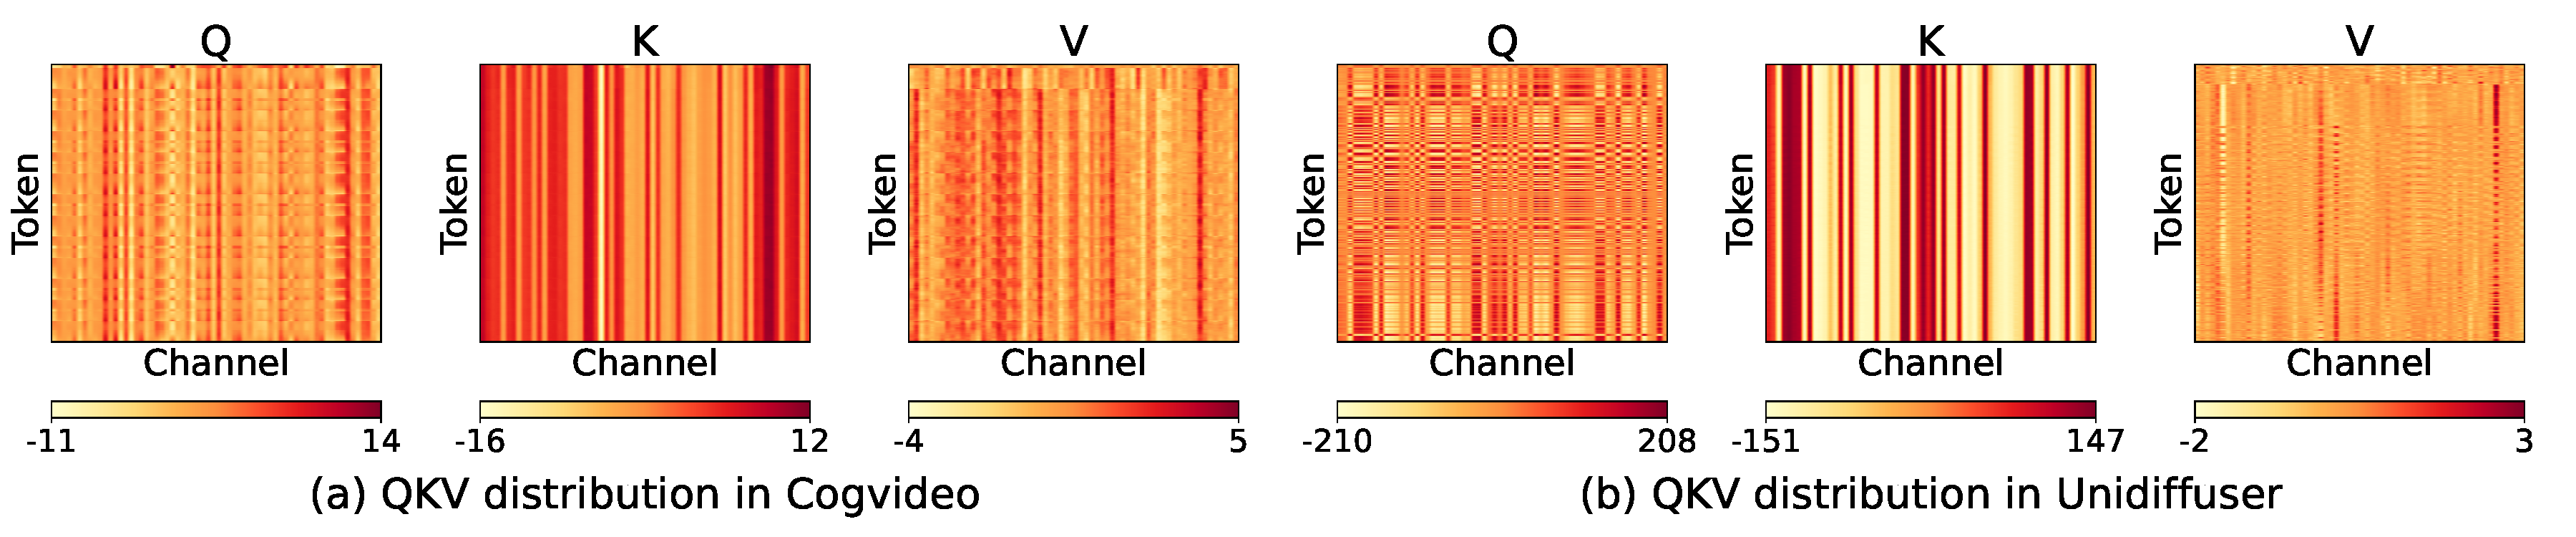
\includegraphics[width=1.0\textwidth]{figs/combined_heatmap.pdf}
    \vspace{-1em}
    \caption{Typical examples of data distribution of (Q, K, V).}
    \end{center}
    \label{fig:heatmap}
\end{figure}

\begin{table}[htb!]
    \caption{End-to-end metrics comparison of different quantization methods.}
    \label{tab:quant_type_analysis}
    \setlength\tabcolsep{2.8pt}
    \begin{center}
    \scalebox{0.97}{
    \begin{tabular}{c|c|c|c|c|c|c}
    \toprule
    \bf\makecell{Quantization \\ (Q, K)} & \bf\makecell{Smoothing \\ K} & \bf\makecell{Llama \\ WikiText} $\downarrow$ & \bf\makecell{CogVideo \\ (Fscore)} $\uparrow$ & \bf\makecell{Unidiffuser \\ (FID)} $\downarrow$ & \bf\makecell{UltraPixel \\ (FID)} $\downarrow$ & \bf\makecell{TIMM \\ ImageNet} $\uparrow$ \\
    \hline
    \bf{Full-Precision} &         -             & 5.823 & 3.768 & 163.33 & 179.78 & 84.79\%    \\ \hline
    \bf\multirow{2}{*}{Per-token}  & \ding{55}  & 5.824 & \dred{1.924} & \dred{221.18} & \dred{193.36} & \dred{84.21\%} \\
                                & \cellcolor{gray!24}\checkmark & \cellcolor{gray!24}5.824 & \cellcolor{gray!24}\textbf{\dgreen{3.734}} & \cellcolor{gray!24}\textbf{\dgreen{166.52}} & \cellcolor{gray!24}\textbf{\dgreen{179.79}} & \cellcolor{gray!24}\dgreen{84.74\%} \\ \hline
    \bf\multirow{2}{*}{Per-block}  & \ding{55}  & 5.825 & \dred{2.014} & \dred{229.08} & \dred{195.67} & \dred{84.18\%} \\
                                & \cellcolor{gray!24}\checkmark & \cellcolor{gray!24}5.824 & \cellcolor{gray!24}\textbf{\dgreen{3.718}} & \cellcolor{gray!24}\textbf{\dgreen{166.93}} & \cellcolor{gray!24}\textbf{\dgreen{179.98}} & \cellcolor{gray!24}\dgreen{84.76\%} \\ \hline
    \bf\multirow{2}{*}{Per-tensor} & \ding{55}  & 5.826 & \dred{1.902} & \dred{267.06} & \dred{196.26} & \dred{84.12\%} \\
                                & \cellcolor{gray!24}\checkmark & \cellcolor{gray!24}5.824 & \cellcolor{gray!24}\textbf{\dgreen{3.640}} & \cellcolor{gray!24}\textbf{\dgreen{167.65}} & \cellcolor{gray!24}\textbf{\dgreen{180.21}} & \cellcolor{gray!24}\dgreen{84.69\%} \\ \hline
    \multicolumn{2}{c|}{\bf FlashAttn3 (with quant)}  & \dred{5.850} &  \dred{3.394}  & \dred{394.13} & \dred{383.61} &  84.70\% \\
    \bottomrule
    \end{tabular}
    }
    \end{center}
\end{table}

\subsection{Smooth Matrix K} \label{sec:smooth_k}
 
Directly quantizing $Q, K$  often results in a large error. Particularly, quantizing $Q, K$ to INT8 yields completely blurry image/video in text-to-image/video tasks. 
As shown in Figure~\ref{fig:heatmap}, we visualize two typical groups of $Q, K, V$ from a text-to-image model \unidiffuser~\citep{bao2022uni} and a text-to-video model \cogvideo~\citep{yang2024cogvideox}. Notably, $K$ exhibits distinct channel-wised outliers. However, per-channel quantization cannot be applied for $K$, because quantization can only be performed at the outer axis (token dim) of the Matmul $QK^\top$. Moreover, the previous smoothing technique proposed for linear layers ~\citep{xiao2023smoothquant} cannot be applied since $Q$ is also heavily affected by outliers. Fortunately, the channel outliers of $K$ have a pattern: Each token's key is actually a \emph{large bias shared by all tokens}, plus a small token-wise signal. Therefore, the outlier is not from large variation across tokens, but simply the large bias. 
Based on this observation, we propose to smooth the matrix $K$ by a transform $\gamma$, which subtracts averaged $K$ across all tokens:
\begin{align} 
    \gamma(K) = K - \mean(K)
\end{align}
where $\mean(K) = \frac{1}{N}\sum_{t=1}^N K[t,:]$ is the average key, with a shape $1\times d$.
Note that such a transformation does not change the attention score $P$, because for any query $q$, we have $\sigma(q (K-\mean(K)^\top)) = \sigma(q K^\top - q\cdot \mean(K)) = \sigma(qK^\top)$. Finally, the transformation from full-precision $K$ to quantized $\hat K$ can be written as $\phi_K(K) = \psi_K\circ \gamma$, where $\psi_K$ is a quantizer. In other words, a full-precision $K$ is substracted with the mean, before eventually being quantized. 


Table~\ref{tab:quant_type_analysis} presents end-to-end metrics for different quantization methods with and without \textit{smoothing K} on various models. The results demonstrate that \textit{smoothing K} offers significant benefits of accuracy. Moreover, the speed overhead of smoothing $K$ for attention is less than \textbf{0.2\%} (See Table\ref{exp:overhead_km}).



\begin{table}[htb!]
    \centering
    \begin{minipage}{0.49\textwidth}
        \raggedright
        \caption{\textbf{Average accuracy} using different data types across all layers of real models.}
        \label{tab:quant_precision_analysis1}
        \setlength\tabcolsep{2.1pt}
        \scalebox{0.91}{
        \begin{tabular}{c|c|c|c|c}
            \toprule
            $Q, K$ & $\widetilde P, V$ & \textbf{Cos Sim $\uparrow$} & \textbf{Relative L1 $\downarrow$} & \textbf{RMSE $\downarrow$} \\
            \hline
            & E4M3 & 99.94\% & 0.0345 & 3.53e-3 \\
            \cellcolor{gray!24}\textbf{INT8} & E5M2 & 99.81\% & 0.0572 & 6.11e-3 \\
                                              & INT8 & 99.70\% & 0.1035 & 6.82e-3 \\
            \hline
            \multirow{3}{*}{E4M3} & E4M3 & 99.81\% & 0.0607 & 5.93e-3 \\
                                              & E5M2 & 99.68\% & 0.0769 & 7.72e-3 \\
                                              & INT8 & 99.58\% & 0.1199 & 8.31e-3 \\
            \hline
            \multirow{3}{*}{E5M2} & E4M3 & 99.37\% & 0.1107 & 1.09e-2 \\
                                              & E5M2 & 99.22\% & 0.1213 & 1.20e-2 \\
                                              & INT8 & 99.13\% & 0.1583 & 1.24e-2 \\
            \bottomrule
        \end{tabular}
        }
    \end{minipage}
    \hspace{0.01\textwidth} 
    \begin{minipage}{0.46\textwidth}
        \raggedleft
        \caption{\textbf{Worst accuracy} using different data types across all layers of real models.}
        \label{tab:quant_precision_analysis2}
        \setlength\tabcolsep{2.1pt}
        \scalebox{0.91}{
        \begin{tabular}{c|c|c|c|c}
            \toprule
            $Q, K$ & $\widetilde P, V$ & \textbf{Cos Sim $\uparrow$} & \textbf{Relative L1 $\downarrow$} & \textbf{RMSE $\downarrow$} \\
            \hline
            \multirow{4}{*}{INT8}  & E4M3 & 76.36\%	   & 0.5899	   & 0.4311 \\
                                   & E5M2 & 78.98\%	& 0.4233	& 0.4371 \\
                                   & INT8 & 56.40\%	& 0.7921	& 0.5405 \\ \cline{2-5}
                                   & \cellcolor{gray!21}\bf{FP16} & \cellcolor{gray!24}\dgreen{99.99\%}	& \cellcolor{gray!24}\dgreen{0.0116}	& \cellcolor{gray!24}\dgreen{0.0091} \\
            \bottomrule
                                       
        \end{tabular}
        }
    \end{minipage}
\end{table}


\subsection{Quantization for Q, K, P, V} \label{sec:qkpv_quant}

\textbf{Quantization granularity for $Q, K$}: 
$\psi_Q(Q)$ and $\psi_K(K)$ can be set with the granularity of per-token, per-block or per-tensor. This is because per-channel quantization is not feasible, since the scale factors of the inner axis of $Q K^\top$ cannot be used to do dequantization~\citep{xiao2023smoothquant}.
 

\textbf{Data type of $Q, K$}: We choose INT8 for $\psi_Q(Q)$ and $\psi_K(K)$ for two reasons. First, Table~\ref{tab:quant_precision_analysis1} shows the average accuracy using different data types (INT8, E4M3, E5M2) for $Q, K, \widetilde P, V$ across all layers of \llama(7B)~\citep{touvron2023llama2} and \unidiffuser. It shows that quantizing $Q, K$ to INT8 performs higher accuracy than using E4M3 and E5M2.
Second, Matmul using INT8 is two times faster than using FP8 in many commonly used GPUs, e.g., RTX4090 and 3090.
 
        

\textbf{Quantization granularity for $\widetilde P, V$}: We propose to use $\psi_P(\widetilde P)$ in per-block and $\psi_V(V)$ in per-channel for three reasons. (1) Per-channel quantization for $\widetilde P$ and per-token quantization for $V$ are not viable because dequantization requires scale factors of the outer axis. (2) $\widetilde P = \mathrm{exp}(S_i - \mathrm{rowmax}(S_i))$, where $S_i$ is the Matmul result of a block of $Q$ and $K^T$, the max value in each row of $\widetilde P$ is 1. Hence, we can assign a single static scale $s = \frac{1}{127}$ to a block $\widetilde P$, whose accuracy equals per-token quantization. (3) Per-channel quantization can address the channel-wised outlier of $V$.

\textbf{Data type of $\widetilde P, V$}: We choose INT8 for $\psi_P(\widetilde P)$ and $\psi_V(V)$ because Matmul using INT8 is two times faster than using FP8 in some commonly used GPUs, and although the accuracy using $\psi_P(\widetilde P)$ and $\psi_V(V)$ in INT8 is worse than E4M3 and E5M2, the average accuracy is similar (See Table~\ref{tab:quant_precision_analysis1}).

\textbf{Accuracy metrics.} We use three metrics to assess the accuracy of quantized attention output $O'$ compared to attention output in full-precision $O$: First, we flatten $O'$ and $O$ into vectors in the shape of $1\times n$. Then, Cosine Sim$=\sum OO' / \smash{\sqrt{\sum O^2}} \smash{\sqrt{\sum O'^2}}$, Relative L1$=\sum |O - O'| / \sum |O|$, RMSE$=\sqrt{(1/n) \sum (O - O')^2}$.

\begin{table}[htb!]
    \centering
    \begin{minipage}{0.46\textwidth}
        \raggedright
        \caption{\textbf{Average accuracy} using different accumulators across all layers of real models.}
        \label{tab:quant_accu_analysis1}
        \setlength\tabcolsep{5pt}
        \scalebox{0.93}{
        \begin{tabular}{c|c|c|c}
            \toprule
            \textbf{Accum.} & \textbf{Cos Sim $\uparrow$} & \textbf{Relative L1 $\downarrow$} & \textbf{RMSE $\downarrow$} \\
            \hline
            \textbf{FP32} & 99.98\% & 0.0156 & 2.94e-3 \\
            \cellcolor{gray!24}\textbf{FP16} & \cellcolor{gray!24}99.98\% & \cellcolor{gray!24}0.0156 & \cellcolor{gray!24}2.94e-3 \\
            \bottomrule
        \end{tabular}
        }
    \end{minipage}
    \hspace{0.025\textwidth} 
    \begin{minipage}{0.5\textwidth}
        \raggedleft
        \caption{\textbf{Worst accuracy} using different accumulators across all layers of real models.}
        \label{tab:quant_accu_analysis2}
        \setlength\tabcolsep{5pt}
        \scalebox{0.93}{
        \begin{tabular}{c|c|c|c}
            \toprule
            \textbf{Accum.} & \textbf{Cos Sim $\uparrow$} & \textbf{Relative L1 $\downarrow$} & \textbf{RMSE $\downarrow$} \\
            \hline
            \textbf{FP32} & 99.84\% & 0.0511 & 4.229e-3 \\
            \cellcolor{gray!24}\textbf{FP16} & \cellcolor{gray!24}99.84\% & \cellcolor{gray!24}0.0511 & \cellcolor{gray!24}4.229e-3 \\
            \bottomrule
        \end{tabular}
        }
    \end{minipage}
\end{table}

\subsection{FP16 accumulator: much more accurate and efficient solution} \label{sec:fp16_acc}

The above solution for $\psi_P(\widetilde P)$ and $\psi_V(V)$ has one problem, that is, the accuracy using INT8 is very poor in some model layers. Table~\ref{tab:quant_precision_analysis2} shows the worst accuracy using different data types for $Q, K, \widetilde P, V$ across all layers
of \llama and \unidiffuser. It shows that INT8 $\psi_P(\widetilde P)$ and $\psi_V(V)$ bring an unacceptable error. 
In response, we propose a very accurate and also efficient solution. Specifically, we propose to use FP16 as the data type of Matmul $\widetilde P V$ with an FP16 accumulator. 

The benefit of such a solution is obvious. First, in the context of some commonly used GPUs, e.g., RTX4090 and 3090, the speed of Matmul in FP16 with an FP16 accumulator is \textbf{2x} faster than that with an FP32 accumulator. Moreover, using FP16 accumulators can save more register resources than using FP32 accumulators, accelerating the computation speed. 
Second, Table~\ref{tab:quant_precision_analysis2} shows that using FP16 for $\widetilde P, V$ is much more accurate than using all the other 8-bit data types. Moreover, using FP16 accumulators incurs no accuracy loss than using FP32 accumulators. Specifically, Table~\ref{tab:quant_accu_analysis1} and~\ref{tab:quant_accu_analysis2} show the average and worst accuracy using FP16 or FP32 accumulators on all layers of \llama and \unidiffuser, showing that there is no accuracy loss of using the FP16 accumulator.


\begin{table}[htb!]
    \centering
    \vspace{-.5em}
    \caption{Four kernel implementations of \our.}
    \label{tab:adaptive_types}
    \setlength\tabcolsep{5pt}
    \scalebox{0.91}{
    \begin{tabular}{c|c|c|c}
        \toprule
        \textbf{Kernel} & $\psi_Q(Q)$, $\psi_K(K)$ & $\psi_P(P)$ & $\psi_V(V)$ \\
        \hline
        \ourt  & per-token, INT8	 & FP16, FP16 Accumulator  & FP16, FP16 Accumulator \\
        \ourb (Algorithm~\ref{alg:ourb}) & per-block, INT8	 & FP16, FP16 Accumulator  & FP16, FP16 Accumulator\\
        \ourvt (Figure~\ref{fig:method_overview}(a)) & per-token, INT8	 & per-block, INT8	       & per-channel, INT8	 \\ 
        \ourvb & per-block, INT8     & per-block, INT8	       & per-channel, INT8 \\
        \bottomrule                  
    \end{tabular}
    }
\end{table}


\begin{figure}[h]
    \begin{center}
    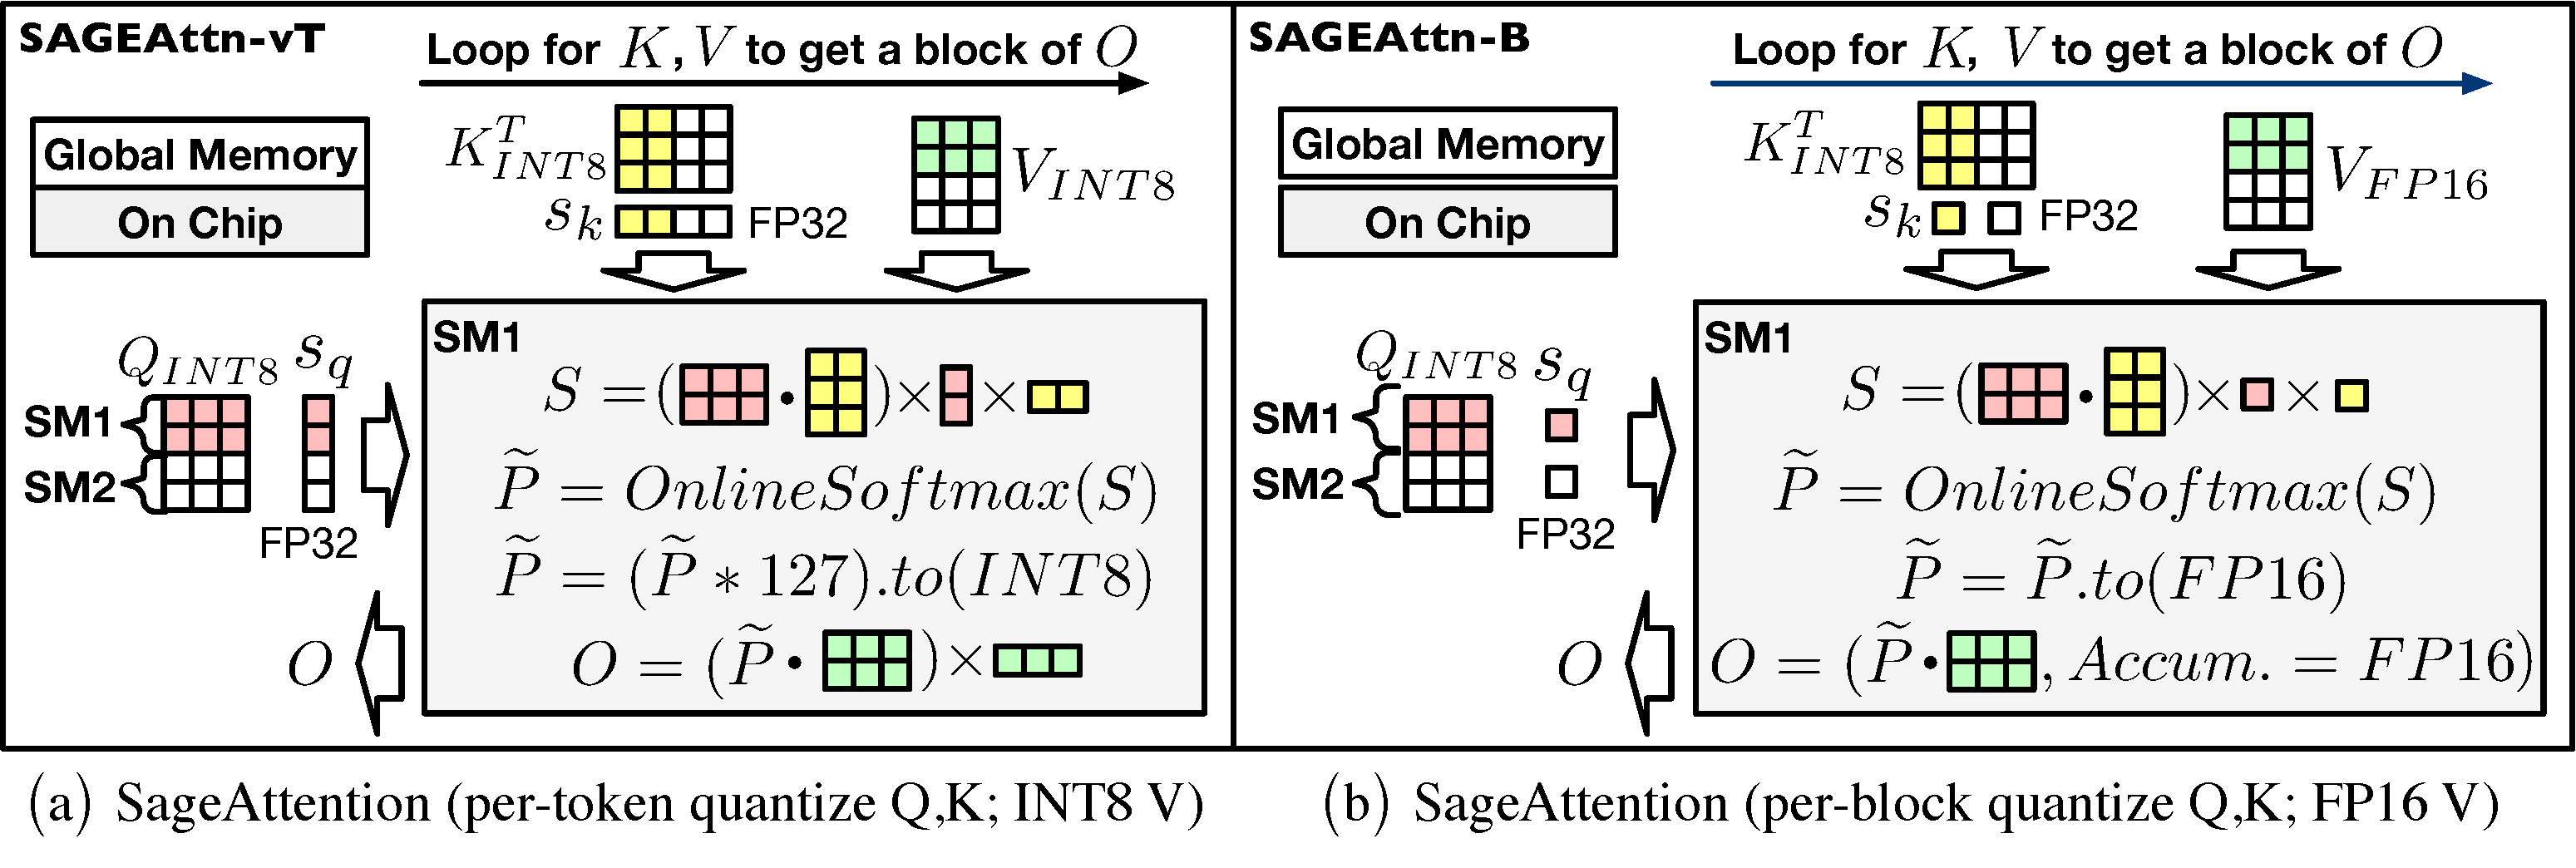
\includegraphics[width=0.95\textwidth]{figs/final_overview.pdf}
    \vspace{-.9em}
    \caption{Workflow of SageAttention.}
    \label{fig:method_overview}
    \end{center}
\end{figure}


\setlength{\textfloatsep}{5pt}
\begin{algorithm}[htb]  
% \SetNoLine
    \small
    \caption{Implementation of \ourb.}
    \label{alg:ourb} 

    \KwIn{Matrices $Q(\text{FP16}), K(\text{FP16}), V(\text{FP16}) \in \mathbb{R}^{N \times d}$, block size $b_q, b_{kv}$.}
    

    \textbf{Preprocessing:} \jt{$K=K-\mathrm{mean}(K)$} ; \tcp{\annotate{Subtracting the mean value across tokens}}

    \textbf{Quantization:} $\jt{(\delta_Q, \hat Q)} = \jt{\psi_Q}(Q/\sqrt{d}),~~\jt{(\delta_K, \hat K)} = \jt{\psi_K}(K)$ ; \tcp{\annotate{INT8 per-block quant}}
    

    Divide \jt{$\hat Q$} into $T_m = {N}/{b_q}$ blocks \jt{$\{\hat Q_i\}$}, and divide \jt{$\hat K$}, $V$ into $T_n = {N}/{b_{kv}}$ blocks \jt{$\{\hat K_i\}$} and $\{V_i\}$;  

    \For (\tcp*{\annotate{Outer loop is paralleled in SMs (stream processors)}}) {$\textbf{i}$ in [1, $T_m$]}{ \vspace{-1em}
        Load \jt{$\hat Q_i$} and \jt{$\delta_Q[i]$} into a SM ;

        \For {$\textbf{j}$ in [1, $T_n$]} { 
            Load \jt{$\hat K_j$}, $V_j$, and \jt{$\delta_K[j]$} into the SM ;

            \jt{$S_i^j = \mathrm{Matmul}(\hat Q_i, \hat K_j^T) \times \delta_Q[i] \times \delta_K[j]$;}

            $m_i^j = \mathrm{max}(m_i^{j-1}, \mathrm{rowmax}(S_i^j))$, $ \widetilde P_i^j = \mathrm{exp}(S_i^j - m_i^j)$, $l_i^j = e^{m_i^{j-1}-m_i^j} l_i^{j-1} + \mathrm{rowsum}(\widetilde P_i^j)$ ;

            $O_i^j = \mathrm{diag}(e^{m_i^{j-1}-m_i^j}) O_i^{j-1} +$ \jt{$\mathrm{Matmul}(\widetilde P_i^j\text{.to(FP16)}, V_j, \text{Accum\_type = FP16})$} ;
        }

        $O_i = \mathrm{diag}(l_i^{T_n})^{-1} O_i^{T_n}$ ;

        Write $O_i$ ;  
    }
    \textbf{return} $O = \{O_i\}$;
\end{algorithm}


\subsection{Adaptive Quantization} \label{sec:adaptive}

Based on the discussion in Section~\ref{sec:qkpv_quant} and ~\ref{sec:fp16_acc}, we implement four attention kernels (See Table~\ref{tab:adaptive_types}) based on two sets of choices: (1) Using $\psi_Q(Q)$ and $\psi_K(K)$ in per-token or per-block. (2) Using $\psi_P(\widetilde P)$ and $\psi_V(V)$ in INT8 or retaining $\widetilde P, V$ in FP16 with an FP16 accumulator.
\purple{\ourb is accurate enough for all models and can achieve a 2x speedup (See Figure~\ref{fig:kf_h64_baseline} and~\ref{fig:kf_h128_baseline}). However, \ourvb is also accurate for some layers in a model and faster a little (about 4\%) than \ourb. Therefore, we use various inputs to test the cosine similarity of \ourvb for each layer of a model. Then, we will select \ourvb for those layers where \ourvb's cosine similarity is bigger than 99.8\% (the worst similarity of \ourb), and the other layers are left for \ourb.}



\subsection{Fusion Tricks and Performance Analysis} \label{sec:fuse_and_performance}

\textbf{Fusion Tricks.} To reduce the overhead of quantization, we fuse the quantization process with the operator preceding the attention layer. For instance, we fuse quantization within the ROPE (Rotary Position Embedding)~\citep{su2021roformer} layer. Specifically, before the ROPE result ($A$) is written from shared memory into global memory, we perform $\delta_A, \hat A = \psi(A)$. Subsequently, the $\delta_A, \hat A$ are written into global memory. Additionally, we also fuse the coefficient ($1/{\sqrt{d}}$) of $Q K^T$ into the quantization process rather than leaving it in the attention layer. Specifically, we multiply $Q$ by ($1/{\sqrt{d}}$) on chip before quantizating $Q$.
\textbf{Performance Analysis.} We will take \ourb as an example to discuss the acceleration effects on actual hardware:
(1) \underline{Matmul acceleration.} Utilizing INT8 matrix multiplication units on current mainstream hardware can achieve \textbf{2-4}$\times$ throughput. While FP16 accumulators do not offer throughput improvements on most compute cards, on-edge accelerators, such as the RTX4090, can still achieve a 2x improvement over FP32 accumulators.
(2) \underline{Quantization overhead.}
Quantization and dequantization are considered the main overhead in current quantization methods~\citep{lin2024qservew4a8kv4quantizationcodesign}. The computational overhead can not be avoided, but through fusing the quantization of $Q, K$ with ROPE, we avoid the IO overhead of quantization. 
(3) \underline{Cache and registers.} Currently, mainstream accelerators need to store data in a cache (such as SharedMemory) during computation. Using 8-bit data for calculations can reduce the usage of the general cache, and using fp16 accumulators can also reduce the usage of accumulation registers. 
(4) \underline{Dram access.} Using 8-bit data can halve the tensors transfer overhead from DRAM to the compute units. Although quantization introduces additional FP32 scales, these scales can be considered negligible compared to the tensors.
